\section{Permutations}
Ladder lotteries and permutations are intricately related to each other. Each $\pi$ has an $OptL\{\pi\}$ such that 
each ladder form $OptL\{\pi\}$ sorts $\pi$. The so called Listing Problem is one of the problems addressed in this thesis.
In brief, this problem is about how to list all $n!$ ladders efficiently. The research for this problem is highly influenced 
by permutation enumeration research. Knuth describes a number of 
permutation enumeration algorithms in The Art of Computer Programming~\cite{A18}. Since this book, many algorithms for 
enumerating $n!$ permutations have been created. During the research for the Listing Problem, twelve of these 
enumeration algorithms were investigated~\cite{A18,A19,A21,A24,A25,A26,A31,A34,A35,A36,A37}.\par 
The first is the lexicographic algorithm which orders all $n!$ permutations from smallest to largest. The lexicographic 
algorithm generates each permutation with an amortized time of $O(n^{2}log(n))$~\cite{A21}. The second of which is the 
colexicographic algorithm which orders all $n!$ permutations from largest to smallest. The colexicographic 
algorithm generates each permutation with an amortized time of $O(n^{2}log(n))$~\cite{A19}. The third of which is Zak's 
algorithm which generates all $n!$ permutations by reversing a suffix in one permutation to get to the next 
permutation. The time complexity of Zak's algorithm is amortized time of $O(n^{2})$~\cite{A31}.
The fourth of which is Heap's algorithm which is a decrease and conquer algorithm.  
The time complexity of Heap's algorithm is {\sc CAT}, constant amortized time of $O(1)$ per permutation~\cite{A24}.
The fifth algorithm is the Steinhaus-Johnson-Trotter algorithm which generates $S_{n}$ by performing adjacent swap operations 
on the permutation resulting in the next permutation. Thus, each permutation in $S_{n}$ differs 
from it predecessor by a single swap operation~\cite{A25}. To go from any two successive permutations, 
the time complexity is $O(1)$~\cite{A25}.
The sixth algorithm is the algorithm using star transpositions that always swaps the first element of the permutation 
with some other element. It was discovered by Gideon Ehrlich and is described as Algorithm E in Knuth's book~\cite{A18}.
The seventh algorithm is the derangement ordering in which no two consecutive permutations have any elements 
in the same position. It was first discussed by Savage in~\cite{A35}. 
The eighth algorithm is the Single Track listing algorithm. Each column in the list of permutations 
is a cyclic shift of the first column~\cite{A36}. The computation for each successive permutation 
is CAT~\cite{A36}.
The ninth algorithm is the Single Track Gray Code listing algorithm. The properties of the Single Track 
listing algorithm hold. Furthermore, any two successive permutations differing by at most two transpositions~\cite{A36}.
The tenth listing algorithm is found in Knuth's book. At each step, it either rotates the permutation to the left by one 
or swaps the first two elements~\cite{A37}. The problem as to whether such a listing algorithm exists for all $n$ 
is posed as an open problem in Knuth's book~\cite{A37}. It was solved by Sawada and Williams in their paper 
A Hamiltonian Path for the Sigma-Tau Problem~\cite{A38}.
The eleventh algorithm is Corbett's algorithm which rotates a prefix of the first possible length in 
$n$,$2$,$n-1$,$3$,$n-2$,$4$, etc.~\cite{A34}. 
The twelfth algorithm is Effler and Ruskey's algorithm which lists permutations by groups of $k$ inversions. %Their algorithm has 
constant amortized time algorithm for generating permutations of order $n$ with $k$ inversions~\cite{A26} meaning 
%the time it takes to generate each permutation is bounded by a constant.
%The algorithm is also a \emph{BEST} algorithm (backtracking ensures success at terminals), meaning that when the algorithm backtracks, 
%the back-tracking leads to a successful result~\cite{A26}. 
To see the listings for all the aforementioned algorithms other than the Effler-Ruskey algorithm, refer to~\ref{Fig:11perms}.\par
\begin{figure} 
    \centering 
    \resizebox{.8\textwidth}{!}{
            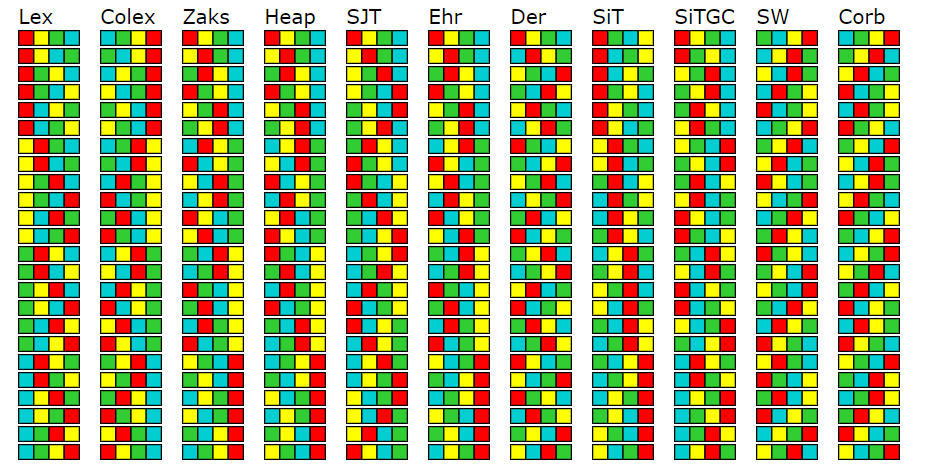
\includegraphics{11perms}
    }
    \caption{Eleven permutation listing algorithms}
    \label{Fig:11perms}
\end{figure}

In Chapter 1, it was stated that Algorithms~\cite{A25}\cite{A26} were the most conducive for The Canonical Ladder Listing Problem. 
These are the Steinhaus-Johnson-Trotter and Effler-Ruskey algorithms respectively. The reason that the SJT algorithm is beneficial 
is because it generates each permutation in $O(1)$ per ladder. In Chapter 3, the SJT 
algorithm is modified to create ladders instead of permutations while still maintaining the same efficiency.
The reason that the Effler-Ruskey algorithm 
is beneficial is because it has a nice ordering property such that the permutations are listed by the number of inversions. In Chapter 3, 
we order all $n!$ ladders by $0,1,2, \dots, {n \choose 2}$ bars where each bar corresponds to an inversion in a permutation.

%Paragraph SJT
\subsection{Steinhaus-Johnson-Trotter Algorithm}
The Steinhaus-Johnson-Trotter algorithm generates $S_{n}$ by performing adjacent swap operations 
on the permutation resulting in the next permutation. Thus, each permutation in $S_{n}$ differs 
from it predecessor by a single swap operation~\cite{A25}. This makes the SJT algorithm a very efficient 
algorithm for listing $S_{n}$. Let an \emph{even permutation} be defined as a permutation 
with an even number of inversion. Let an \emph{odd permutation} be defined as a 
permutation with an odd number of inversions. The $nth$ element is inserted into all 
positions of $\pi$ of order $n-1$ in descending order if $\pi$ of order $n-1$ is an even permutation.
The $nth$ element is inserted into all positions of $\pi$ of order $n-1$ in ascending order if 
$\pi$ of order $n-1$ is an odd permutation~\cite{A25}. For $\pi$ of order $1$ we have $\pi=(1)$. Since 
there are no inversions in $\pi=(1)$ it is even. Now insert $2$ in all positions in $\pi=(1)$
in descending order. Thus we get $(1,2)$ followed by $(2,1)$. Since $(1,2)$ is 
an even permutation, insert $3$ into all positions in descending order resulting in $(1,2,3)$,
$(1,3,2)$ and $(3,1,2)$. Since $(2,1)$ is an odd permutation, insert $3$ 
into all permutations in ascending order resulting in $(3,2,1)$, $(2,3,1)$ and $(2,1,3)$.
Initialize $\pi$ to the identity permutation, initialize $currentElement$ to $2$, initialize 
$n$ to $p_{max}$. Let $direction$ be a Boolean array of size $n$ initialized to $true/right$ for indices. 
If $currentElement$ is greater than $n$, print $\pi$ 
and return. Otherwise, begin a for loop that runs $i=[1 \dots n-1]$ times. 
In the for loop, first make a recursive call with $currentElement$ increasing by one. 
If $direction[currentElement]$ is $right$, then swap $currentElement$ in $\pi$ with its left neighbor. Else 
if $direction[currentElement]$ is $left$ then swap the $currentElement$ in $\pi$ with its right neighbor.
Once the for loop has exited, make one more recursive call with $currentElement+1$ outside the for loop; 
this avoids an extra swap operation from occurring while still maintaining the correct number of recursive 
calls. Lastly, negate $direction[currentElement]$, which effectively changes the direction of the $currentElement$ 
in $direction$ for the next time $currentElement$ is to be swapped. 
To see the Steinhaus-Johnson-Trotter algorithm please refer to Algorithm~\ref{Alg:SJT}.

\begin{algorithm}
    \begin{algorithmic}[1]
        \Function{SJT}{$\pi$, $currentElement$, $n$, $direction$}
            \If{$currentElement > n$}
                \If{{\sc Sorted($\pi$)}}
                    \State {\sc Print($\pi$)}
                \EndIf
                \State \textbf{return}
            \EndIf
            \For{$i$ \textbf{from} $1$ \textbf{to} $currentElement-1$}
                \State {\sc SJT($\pi$, $currentElement+1$, $n$)}
                \State $index \gets $ index of $currentElement$ in $\pi$
                \If{$direction[currentElement]=right$}
                    \State {\sc Swap}$(p_{index}, p_{index-1})$
                \Else 
                    \State {\sc Swap}$(p_{index}, p_{index+1})$
                \EndIf
                \State {\sc Print}$(\pi)$
            \EndFor
            \State {\sc SJT}($\pi$, $currentElement+1$, $n$, $direction$)
            \If{$direction[currentElement]=right$}
                \State $direction[currentElement] \gets left$
            \Else 
                \State $direction[currentElement] \gets right$
            \EndIf
        \EndFunction
        
    \end{algorithmic}
    \caption{SJT Algorithm for listing $S_{n}$}
    \label{Alg:SJT}
\end{algorithm}

The Steinhaus-Johnson-Trotter algorithm is a Gray Code, meaning that in order to transition 
between any two subsequent permutations in $S_{n}$, there is a minimal amount of constant 
change required. The algorithm simply swaps two elements in order to transition between 
permutations. Each recursive call creates a new permutation with the exception of the 
initial call to the function in which $n$ recursive calls need to be made before the 
first permutation is printed. The amortized time to transition between permutations is $O(1)$.




%%Paragraph 
\subsection{Effler-Ruskey Algorithm}
%%%%%%%%%%FIX ME %%%%%%%%%%%%%%%%
In the paper A CAT Algorithm for Generating Permutations with a Fixed Number of Inversions, written by Effler and Ruskey, the authors provide a 
constant amortized time algorithm for generating all permutations of order $n$ with $k$ inversions~\cite{A26} meaning 
the time it takes to generate each permutation is bounded by a constant.
The algorithm is also a \emph{BEST} algorithm (backtracking ensures success at terminals), meaning that when the algorithm backtracks, 
the back-tracking leads to a successful result~\cite{A26}. 
Let the initial conditions of the algorithm be the following. Let $\pi$ be the empty permutation of order $n$. Let $n$
be initialized as the elements $[1 \dots n]$. Let $k$ be initialized to an integer between $[0 \dots {n \choose 2}]$. 
Let $list$ be initialized to the list of $n$ elements in strictly descending order. 
Let $i$ be the index of element $x$ in $list$. $n-i$ 
indicates the number of inversions formed with $x$ when inserting $x$ into position $n$ in $\pi$.
The algorithm works as follows.
Going right to left in the $list$, each element, $x$, in $list$ is inserted into $p_{n}$
only if inserting $x$ into position $n$ in $\pi$ does not exceed the current number of inversions, $k$. I.E. only 
if $k- (n-i) \geq 0$.
If $x$ is inserted into $\pi$ at position $n$ then $x$ is removed from $list$, a recursive call is made such that $n$ is reduced by 
$1$ and $k$ is reduced by $(n-i)$. When the function returns from its recursive call, element $x$ is placed back into the list 
at its original position. To see the algorithm please refer to Algorithm~\ref{Alg:KInv}.\pagebreak
\begin{algorithm}[t]
    \begin{algorithmic}[1]
        \Function{KInversions}{$\pi$, $n$, $k$, $list$}
            \If{$n = 0$ and $k = 0$}
                \State {\sc Print}($\pi$)
            \Else
                \For{$i$ \textbf{from} length \textbf{of} $list$ \textbf{to} $1$}
                    \State $x \gets list_{i}$
                    \If{$n-i \leq k \leq {n-1\choose k} + (n-i)$}
                        \State $p_{n} \gets x$
                        \State remove $x$ from $list$ 
                        \State $k \gets k - (n-i)$
                        \State {\sc KInversions}$(\pi, n-1, k, list)$
                        \State insert $x$ in $list$ at correct position.
                    \EndIf
                \EndFor
            \EndIf
        \EndFunction
        
    \end{algorithmic}
    \caption{Generate all permutations with $k$ inversions}
    \label{Alg:KInv}
\end{algorithm} 

Below is an example of how the algorithm creates one permutation of order $4$ with $2$ inversions.
\begin{enumerate}
    \item Initial Call: {\sc KInversions}($\pi$=(\underline{ },\underline{ },\underline{ },\underline{ }),$n=4$,$k=2$,$list=[1,2,3,4]$):\newline 
    given $\pi$=(\underline{ },\underline{ },\underline{ },\underline{ }), $n=4$, $k=2$, $list=[1,2,3,4]$, $i=2$ and $x=3$ 
    then inserting $x$ into position $n=4$ would form $4-3=1$ 
    inversion(s). Specifically, the inversion $(4,3)$. Thus, $k$ would be reduced by $1$ in the recursive call 
    and $n$ would be reduced by $1$ in the recursive call. 

    \item First recursive call: {\sc KInversions}($\pi$=(\underline{ },\underline{ },\underline{ },\underline{3}),$n=3$,$k=1$,$list=[1,2,4]$):\newline 
    given $\pi$=(\underline{ },\underline{ },\underline{ },\underline{3}),$n=3$,$k=1$,$list=[1,2,4]$,$i=3$ and $x=4$
    then inserting $x$ into position $3$ would form $3-3=0$ inversions. Thus, $k$ would be reduced by $0$ in the 
    recursive call and $n$ would be reduced by $1$ in the recursive call.

    \item Second recursive call: {\sc KInversions}($\pi$=(\underline{ },\underline{ },\underline{4},\underline{3}),$n=2$,$k=1$,$list=[1,2]$):\newline 
    given $\pi$=(\underline{ },\underline{ },\underline{4},\underline{3}),$n=2$,$k=1$,$list=[1,2]$,$i=1$ and $x=1$
    then inserting $x$ into position $1$ would form $2-1=1$ inversion. Thus, $k$ would be reduced by $1$ to $0$ in the 
    recursive call and $n$ would be reduced by $1$ in the recursive call.

    \item Third recursive call: {\sc KInversions}($\pi$=(\underline{ },\underline{1},\underline{4},\underline{3}),$n=1$,$k=0$,$list=[2]$):
    \newline given $\pi$=(\underline{ },\underline{1},\underline{4},\underline{3}), $n=1$, $k=0$, $list=[2]$ $i=1$ and $x=2$
    then inserting $x$ into position $1$ would form $1-1=0$ inversions. Thus, $k$ would be reduced by $0$
    and $n$ would be reduced by $1$.

    \item Fourth recursive call: {\sc KInversions}($\pi$=(\underline{2},\underline{1},\underline{4},\underline{3}),$n=0$,$k=0$,$list=[]$):\newline 
    Given $n=0$ and $k=0$ the algorithm {\sc Prints}($\pi$) and returns.
\end{enumerate}


